\documentclass[11pt]{article}

\usepackage[margin=1in]{geometry}
\usepackage{amsmath}
\usepackage{graphicx}
\usepackage{booktabs}
\usepackage{float}
\usepackage{caption}


\title{Homework 2 CS 555 Spring 26}
\author{Md Istiaque Ahmed (miahmed2)} 
\date{\today}

\begin{document}

\maketitle

\section*{Question 1: 1D Burgers Equation}

In this problem, we numerically solve the 1D Burgers equation:
\begin{equation}
    \frac{\partial u}{\partial t} + u\frac{\partial u}{\partial x} = \nu\frac{\partial^2 u}{\partial x^2}
\end{equation}
on the domain $\Omega = [0,1]$ with homogeneous Dirichlet boundary conditions and initial condition $u^0(x) = \sin(\pi x)$. The viscosity is set to $\nu = 1/(100\pi)$.

\subsection*{Part (a): Solution Snapshots}
The equation is integrated using finite differences with 3-point stencils for spatial derivatives and a 3rd-order Implicit-Explicit (IMEX) scheme in time (BDF3 for the viscous term, EXT3 for the convective term). The time-stepping is bootstrapped using 1st and 2nd-order methods for the initial two steps. 

Figure \ref{fig:snapshots} displays the computed solution profile $u(x,t)$ at intervals of $0.1$ up to $t=2.0$. As expected, the initial sine wave advects to the right and steepens, forming a sharp boundary layer against the wall at $x=1$.

\begin{figure}[H]
    \centering
    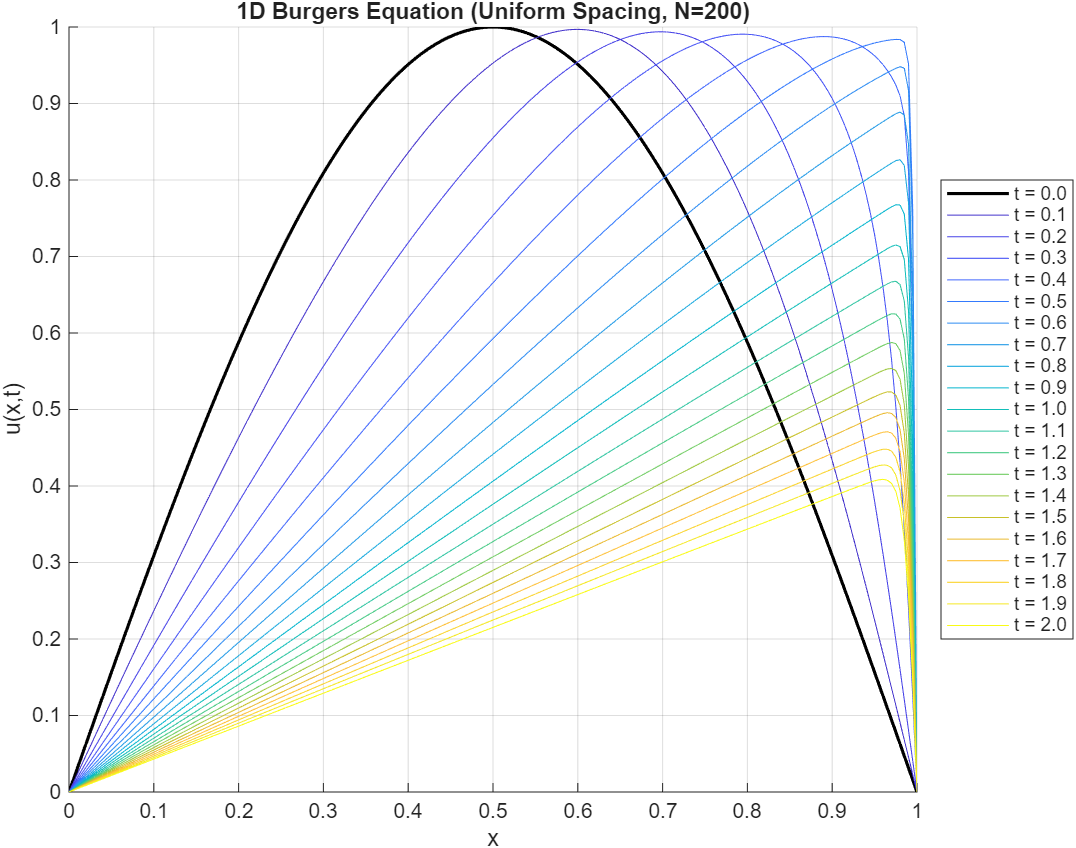
\includegraphics[width=0.8\textwidth]{snapshots.png}
    \caption{Evolution of the 1D Burgers equation on a uniform grid ($N=200$). Snapshots are taken every $0.1$ seconds.}
    \label{fig:snapshots}
\end{figure}

\subsection*{Part (b): Maximum Spatial Derivative}
We compute $s(t) = \max | \partial u / \partial x |$ over the domain for $t \in [0,2]$. The time step is chosen to satisfy $\text{CFL} = 0.1$. Assuming a maximum wave speed of $|c| \approx 1.0$ and uniform spacing $\Delta x = 1/200$, this yields a stable timestep of $\Delta t = 0.0005$. The computed parameters for the uniform grid ($N=200$) are:
\begin{itemize}
    \item \textbf{Maximum slope:} $s^* = 208.77638$
    \item \textbf{Time of maximum:} $t^* = 0.51400$
\end{itemize}

Figure \ref{fig:max_slope} visualizes the evolution of this derivative. The qualitative behavior agrees with Figure 6 in the Basdevant et al. reference paper, exhibiting a rapid spike to a maximum value followed by a gradual viscous decay. Because Figure 6 is plotted against $\pi t$, our peak occurring at $t \approx 0.51$ correctly aligns with their reported peak near $\pi t \approx 1.6$. 

Comparing our numerical values to Table 3 of the reference (analytical $s^* \approx 152.005$ at $t^* \approx 0.51$), the temporal location $t^*$ is highly accurate. However, the computed magnitude $s^*$ exhibits a significant overshoot ($208.78$ vs. $152.00$). This discrepancy is a direct consequence of numerical dispersion; the uniform spacing of $\Delta x = 1/200$ is too coarse to adequately resolve the boundary layer, introducing non-physical, spurious oscillations that artificially inflate the maximum derivative.

\begin{figure}[H]
    \centering
    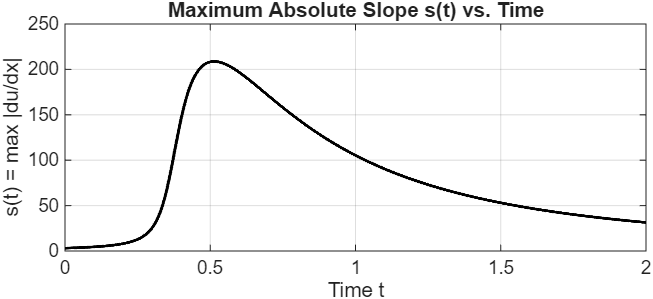
\includegraphics[width=0.8\textwidth]{max_slope.png}
    \caption{Maximum absolute spatial derivative $s(t)$ versus time.}
    \label{fig:max_slope}
\end{figure}

\subsection*{Part (c): Convergence with Uniform Spacing}
We compute $s^*$ as a function of $N=2^k$ for $k=5, 6, \dots, 11$ using uniform spacing and the convective formulation. The tabulated relative errors against the analytical maximum $s^* = 152.00516$ are presented in Table \ref{tab:part_c}. 

\begin{table}[H]
\centering
\caption{Convergence of $s^*$ for Uniform Spacing (Convective Form)}
\label{tab:part_c}
\begin{tabular}{@{}rrrr@{}}
\toprule
$N$ & nsteps & $s^*$ & rel.err. \\
\midrule
  32 &   640 & 204.75163 & $3.47004 \times 10^{-1}$ \\
  64 &  1280 & 264.95618 & $7.43074 \times 10^{-1}$ \\
 128 &  2560 & 241.56922 & $5.89217 \times 10^{-1}$ \\
 256 &  5120 & 192.58263 & $2.66948 \times 10^{-1}$ \\
 512 & 10240 & 164.69320 & $8.34711 \times 10^{-2}$ \\
1024 & 20480 & 155.38910 & $2.22620 \times 10^{-2}$ \\
2048 & 40960 & 152.86551 & $5.66003 \times 10^{-3}$ \\
\bottomrule
\end{tabular}
\end{table}

\subsection*{Part (d): Conservation Form at Finest Resolution}
The nonlinear advection term can be recast into the conservation form: $\frac{1}{2}\frac{\partial u^2}{\partial x}$. Testing this approach at the finest uniform resolution ($N=2048$, $\Delta t \approx 4.88 \times 10^{-5}$) yields:
\begin{itemize}
    \item \textbf{Maximum slope:} $s^* = 152.42586$
    \item \textbf{Time of maximum:} $t^* = 0.51050$
\end{itemize}
While the physical formulations are analytically equivalent, the discrete truncation error differs from the convective form, resulting in a slightly modified approximation of the maximum slope.

\subsection*{Part (e): Convergence Study and Comparison}

The following tables document the convergence behavior for $N=2^k$ ($k=5, \dots, 11$) across four combinations of spatial discretization and nonlinear formulation. As instructed, the timestep $\Delta t = 0.1/N$, derived from the uniform grid CFL condition, is held constant across all cases to ensure a direct comparison without introducing variable time-stepping artifacts. The convergence ratio is defined as $\text{err}_{N/2}/\text{err}_{N}$.

\begin{table}[H]
\centering
\caption{Case i. Uniform spacing, convective form}
\begin{tabular}{@{}rrrrr@{}}
\toprule
$N$ & nsteps & $s^*$ & rel.err. & ratio \\
\midrule
  32 &   640 & 204.75163 & $3.47004 \times 10^{-1}$ & - \\
  64 &  1280 & 264.95618 & $7.43074 \times 10^{-1}$ & 0.467 \\
 128 &  2560 & 241.56922 & $5.89217 \times 10^{-1}$ & 1.261 \\
 256 &  5120 & 192.58263 & $2.66948 \times 10^{-1}$ & 2.207 \\
 512 & 10240 & 164.69320 & $8.34711 \times 10^{-2}$ & 3.198 \\
1024 & 20480 & 155.38910 & $2.22620 \times 10^{-2}$ & 3.749 \\
2048 & 40960 & 152.86551 & $5.66003 \times 10^{-3}$ & 3.933 \\
\bottomrule
\end{tabular}
\end{table}

\begin{table}[H]
\centering
\caption{Case ii. Chebyshev spacing, convective form}
\begin{tabular}{@{}rrrrr@{}}
\toprule
$N$ & nsteps & $s^*$ & rel.err. & ratio \\
\midrule
  32 &   640 & 167.45688 & $1.01653 \times 10^{-1}$ & - \\
  64 &  1280 & 153.42089 & $9.31369 \times 10^{-3}$ & 10.914 \\
 128 &  2560 & 152.11972 & $7.53643 \times 10^{-4}$ & 12.358 \\
 256 &  5120 & 152.01843 & $8.72962 \times 10^{-5}$ & 8.633 \\
 512 & 10240 & 152.00751 & $1.54404 \times 10^{-5}$ & 5.654 \\
1024 & 20480 & 152.00569 & $3.48080 \times 10^{-6}$ & 4.436 \\
2048 & 40960 & 152.00529 & $8.50164 \times 10^{-7}$ & 4.094 \\
\bottomrule
\end{tabular}
\end{table}

\begin{table}[H]
\centering
\caption{Case iii. Uniform spacing, conservation form}
\begin{tabular}{@{}rrrrr@{}}
\toprule
$N$ & nsteps & $s^*$ & rel.err. & ratio \\
\midrule
  32 &   640 &  65.52165 & $5.68951 \times 10^{-1}$ & - \\
  64 &  1280 & 102.90704 & $3.23003 \times 10^{-1}$ & 1.761 \\
 128 &  2560 & 140.71434 & $7.42792 \times 10^{-2}$ & 4.348 \\
 256 &  5120 & 157.73907 & $3.77218 \times 10^{-2}$ & 1.969 \\
 512 & 10240 & 156.53456 & $2.97977 \times 10^{-2}$ & 1.266 \\
1024 & 20480 & 153.55362 & $1.01869 \times 10^{-2}$ & 2.925 \\
2048 & 40960 & 152.42586 & $2.76767 \times 10^{-3}$ & 3.681 \\
\bottomrule
\end{tabular}
\end{table}

\begin{table}[H]
\centering
\caption{Case iv. Chebyshev spacing, conservation form}
\begin{tabular}{@{}rrrrr@{}}
\toprule
$N$ & nsteps & $s^*$ & rel.err. & ratio \\
\midrule
  32 &   640 & 159.19227 & $4.72820 \times 10^{-2}$ & - \\
  64 &  1280 & 153.81930 & $1.19348 \times 10^{-2}$ & 3.962 \\
 128 &  2560 & 152.15108 & $9.59988 \times 10^{-4}$ & 12.432 \\
 256 &  5120 & 152.01876 & $8.94915 \times 10^{-5}$ & 10.727 \\
 512 & 10240 & 152.00711 & $1.28268 \times 10^{-5}$ & 6.977 \\
1024 & 20480 & 152.00556 & $2.62221 \times 10^{-6}$ & 4.892 \\
2048 & 40960 & 152.00525 & $6.23135 \times 10^{-7}$ & 4.208 \\
\bottomrule
\end{tabular}
\end{table}

\subsubsection*{Discussion}
\begin{itemize}
    \item \textbf{Grid Spacing (Uniform vs. Chebyshev):} The uniform grid severely under-resolves the sharp internal layer at lower $N$ values, leading to significant numerical dispersion. This manifests as poor approximations of $s^*$ and erratic error convergence until $N \ge 1024$. In contrast, Chebyshev spacing naturally clusters grid points at the boundaries, placing high resolution precisely where the local gradients are maximized. Consequently, the Chebyshev cases reach an $\approx 10^{-5}$ relative error by just $N=256$, outperforming the uniform grid's finest resolution.
    \item \textbf{Convergence Ratio:} The theoretical error ratio for a second-order scheme when halving the spatial step size is $\approx 4$. For the Chebyshev grids (Cases ii and iv), the ratio rapidly stabilizes and approaches $\approx 4.1$ by the finest resolution, strictly confirming the scheme's second-order spatial accuracy. For uniform grids, the ratio behaves erratically before finally approaching the theoretical asymptotic value once the grid properly resolves the boundary layer at high $N$.
    \item \textbf{Formulation (Convective vs. Conservation):} At lower resolutions, the discrete truncation errors of the two forms lead to distinct failure modes; the convective form overestimates $s^*$ due to spurious oscillations, while the conservation form under-predicts it. However, once the grid is sufficiently refined (especially with Chebyshev spacing), both formulations converge to the analytical maximum $s^* \approx 152.005$ with nearly identical precision, robustly validating their formal equivalence.
\end{itemize}

\end{document}